\documentclass[a4paper,ngerman]{scrartcl}

\usepackage[utf8]{inputenc}
\usepackage[ngerman]{babel}
\usepackage{amsmath,amsthm,amssymb,amscd,color,graphicx,environ,mathtools}
\usepackage{framed}
\usepackage[protrusion=true,expansion=true]{microtype}
\usepackage{lmodern}
\usepackage{multicol}
\usepackage[normalem]{ulem}
\usepackage{hyperref}

\newcommand{\defeq}{\vcentcolon=}

\usepackage[paperwidth=184mm,paperheight=297mm]{geometry}
%\geometry{tmargin=2cm,bmargin=2cm,lmargin=2cm,rmargin=2cm,width=10cm}

\usepackage{canoniclayout}

\setlength{\unitlength}{1cm}

\setlength\parskip{\medskipamount}
\setlength\parindent{0pt}

\renewcommand*\theenumi{\alph{enumi}}
\renewcommand{\labelenumi}{\theenumi)}

\newlength{\aufgabenskip}
\setlength{\aufgabenskip}{1.4em}
\newcounter{aufgabennummer}
\newenvironment{aufgabe}[1]{
  \addtocounter{aufgabennummer}{1}
  \textbf{Aufgabe \theaufgabennummer.} \emph{#1} \par
}{\vspace{\aufgabenskip}}
\newenvironment{aufgabeE}[1]{\begin{aufgabe}{#1}\begin{enumerate}}{\end{enumerate}\end{aufgabe}}

\clubpenalty=10000
\widowpenalty=10000
\displaywidowpenalty=10000

\newcommand{\NN}{\mathbb{N}}
\newcommand{\RR}{\mathbb{R}}
\DeclarePairedDelimiter{\floor}{\lfloor}{\rfloor}

\begin{document}

Institut für Mathematik \\
Universität Augsburg

\begin{center}
  \textbf{Übungsblatt zur Vorlesung} \\
  \emph{Geheimnis der Zahl 5}
\end{center}
\vspace{1em}

\begin{aufgabe}{Ein Kästchen verschwindet!}
\begin{enumerate}
\item Die beiden Figuren bestehen offensichtlich aus denselben Stücken, haben
aber unterschiedlichen Flächeninhalt! Was ist hier passiert?
\item Zeige: Der Quotient zweier aufeinanderfolgender Fibonacci-Zahlen nähert
sich beliebig genau dem goldenen Schnitt an.
\end{enumerate}
\begin{center}
  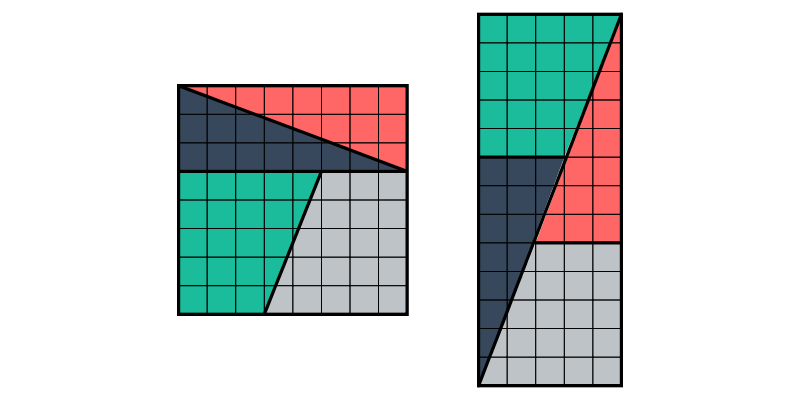
\includegraphics[scale=0.3]{ein-kaestchen-verschwindet}
\end{center}
\end{aufgabe}

\begin{aufgabe}{Die Quadrate der Fibonacci-Zahlen}
Es gilt die Identität~$\sum_{i=0}^n f_i^2 = f_n f_{n+1}$.
\begin{enumerate}
\item Führe einen Induktionsbeweis.
\item Argumentiere, wieso folgende Skizze die Behauptung auch schon beweist.
\end{enumerate}
\begin{center}
  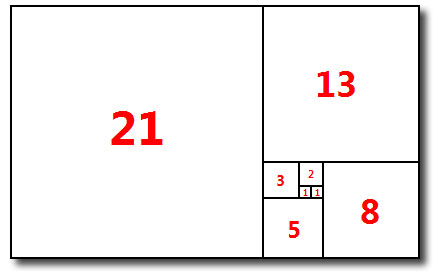
\includegraphics[scale=0.3]{fibonacci-quadrate}
\end{center}
\end{aufgabe}

\begin{aufgabe}{Irrationalste Zahl}
Formuliere präzise und beweise: Der goldene Schnitt ist die irrationalste Zahl.

\emph{Tipp:} Kettenbruchentwicklung.
\end{aufgabe}

\begin{aufgabe}{Ableitung vs. Umkehrfunktion}
Finde eine bijektive differenzierbare Funktion~$\RR^+ \to \RR^+$, deren
Ableitung gleich ihrer Umkehrfunktion ist.
\end{aufgabe}

\begin{aufgabe}{Conways Armee}
Ein unendlich ausgedehntes Damebrett sei in zwei Hälften zerteilt. Im unteren
Teil darf man beliebig viele Damesteine platzieren. Ziel des Spiels ist es,
einen Damestein möglichst hoch in das obere Spielfeld zu
bringen. Dabei darf nur folgender Spielzug angewendet werden: Ein Stein
darf einen (horizontal oder vertikal) benachbarten Stein überspringen, wenn das
Zielfeld unbesetzt ist. Der übersprungene Stein wird dann aus dem Spiel
entfernt.
\begin{enumerate}
\item Überzeuge dich davon, dass man, um Höhe~1, 2, 3 bzw. 4 über der
Trennlinie zu erreichen, mit~2, 4, 8 bzw. \sout{16} 20 Steinen beginnen muss.
\item Zeige, dass Höhe~5 mit keiner endlichen Anzahl von Steinen erreichbar
ist.

\emph{Tipp:} Weise den Spielsteinen eine von der Manhattan-Entfernung zum
angepeilten Zielstein abhängige Bewertung zu.
\end{enumerate}
\end{aufgabe}

\begin{aufgabe}{Auflösbarkeit quintischer Gleichungen}
Zeige, dass Gleichungen vom Grad~5 und höher im Allgemeinen nicht durch
Radikale auflösbar sind.

\emph{Tipp:} Eine Gleichung ist genau dann durch Radikale auflösbar, wenn die
zugehörige Galoisgruppe eine auflösbare Gruppe ist. Wenn man daher zeigt, dass
die symmetrische Gruppe in~$n$ Ziffern für $n \geq 5$ nicht auflösbar ist, hat
man schon viel gewonnen.
\end{aufgabe}

\begin{aufgabe}{Eine Zahl mit besonderer Dezimalbruchentwicklung}
Es gilt:
\[ \frac{1}{998999} =
  0{,}000\,001\,001\,002\,003\,005\,008\,013\,021\ldots. \]
\begin{enumerate}
\item Was ist daran besonders?
\item Inwiefern setzt sich das Muster auch nach~$987$ fort?
\item Erkläre das Phänomen.
\end{enumerate}
\end{aufgabe}

\begin{aufgabe}{Willmore-Satz}
Kathrin und Meru, ihr seid gefragt!
\end{aufgabe}

\begin{aufgabe}{Ein Lemma über goldene Dreiecke}
\begin{enumerate}
\item Zeige: In einem gleichschenkligen Dreieck mit den
Innenwinkeln~$72^\circ$, $36^\circ$ und~$72^\circ$ teilen die langen Seiten die
Grundseite im goldenen Schnitt.
\item Beweise damit folgende Pentagon-Dekagon-Hexagon-Identität: Seien ein
reguläres Pentagon, ein reguläres Dekagon und ein reguläres Hexagon in einem
Kreis einbeschrieben. Dann gilt für die Kantenlängen~$P$,~$D$ bzw.~$H$ die
Identität $P^2 = D^2 + H^2$.
\end{enumerate}
\end{aufgabe}

\begin{aufgabe}{Ikosaeder und Dodekaeder}
Sei einem regelmäßigen Ikosaeder ein regelmäßiges Dodekaeder einbeschrieben
(Seitenflächenmittelpunkte auf Ecken). Zeige, dass das Verhältnis der Kantenlängen
beider Objekte gleich $3:\Phi$ ist.
\end{aufgabe}

\begin{aufgabe}{Rotation um $72^\circ$}
\begin{enumerate}
\item Zeige: Die dreidimensionale Rotation um $72^\circ = \frac{2\pi}{5}$ hat Spur~$\Phi$.
\item Zeige: Die zweidimensionale Rotation um~$72^\circ$ hat Spur~$\frac{1}{\Phi}$.
\end{enumerate}
\end{aufgabe}

\begin{aufgabe}{Ein naiver Algorithmus für Fibonacci-Zahlen}
Eine ganz naive Methode, die~$n$-te Fibonacci-Zahl zu bestimmen, besteht
darin, die beiden Vorgänger zu bestimmen und dann zu summieren. Wie viele
Rechenschritte sind dabei notwendig, wenn man sich \emph{nicht}
Zwischenergebnisse merkt und daher viele Fibonacci-Zahlen immer wieder
berechnet?
\end{aufgabe}

\begin{aufgabe}{Erzeugende Funktionen für Fibonacci-Zahlen}
\begin{enumerate}
\item Zeige, dass die gewöhnliche und exponentiell erzeugende Funktionen der
Fibonacci-Zahlen durch
\begin{align*}
  \sum_{n\geq 0} f_{n+1}x^n &= \frac{1}{1-x-x^2} \qquad\text{bzw.} \\
  \sum_{n\geq 0} \tfrac{1}{n!}f_n x^n &= \tfrac{1}{\sqrt{5}}\exp\left(\tfrac{1+\sqrt{5}}{2}\, x\right) - \tfrac{1}{\sqrt{5}}\exp\left(\tfrac{1-\sqrt{5}}{2}\, x\right)
\end{align*}
gegeben sind.
\item Zeige weiter:
\begin{align*}
\sum_{n\geq 0} f_{n+1}^2x^n &= \frac{2}{5}\cdot\frac{1}{1+x}\ +\ \frac{1}{5}\cdot\frac{3-2x}{1-3x+x^2}\\
\sum_{n\geq 0} f_{n+1}^3x^n &= \frac{3}{5}\cdot\frac{1}{1+x-x^2}\ +\ \frac{2}{5}\cdot\frac{1}{1-4x-x^2} \\
\sum_{n\geq 0} f_{n+1}^4x^n &= \frac{6}{25}\cdot\frac{1}{1-x}\ +\ \frac{4}{25}\cdot\frac{3+2x}{1+3x+x^2}\ +\ \frac{1}{25}\cdot\frac{7-2x}{1-7x+x^2}\\
\sum_{n\geq 0} f_{n+1}^5x^n &= \frac{2}{5}\cdot\frac{1}{1-x-x^2}\ +\ \frac{2}{5}\cdot\frac{1}{1+4x-x^2}\ +\ \frac{1}{5}\cdot\frac{1}{1-11x-x^2}
\end{align*}
Die einzelnen Summanden haben alle eine besondere Bedeutung. Welche? Wie lautet
die erzeugende Funktion einer beliebigen Potenz von Fibonacci-Zahlen?
\end{enumerate}
\end{aufgabe}

\begin{aufgabe}{Wallsche Vermutung}
Bekanntlich gilt~$f_5 = 5$. Allgemeiner gibt es für jede positive Zahl~$k$ eine
positive Zahl~$r$ sodass~$f_{r \NN} \subseteq k \NN$. Sei die kleinste solche
Zahl~$r(k)$. Beweise oder widerlege: Für Primzahlen~$p$ gilt~$r(p^\ell) =
p^{\ell-1} r(p)$. Insbesondere ist~$f_{5^\ell}$ stets durch~$5$ teilbar.
\end{aufgabe}

\begin{aufgabe}{Fibonacci-Zahlen als Permanente}
Zeige: Die Permanente einer~$(n \times n)$-Bandmatrix, die auf der
Hauptdiagonale und den beiden Nebendiagonalen mit Einsern und sonst nur mit
Nullern besetzt ist, ist~$f_{n+1}$.
\end{aufgabe}

\begin{aufgabe}{Semistabilität von Vektorbündeln [Andrei Okounkov]}
Sei $E$ ein Vektorbündel auf $\mathbb{CP}^2$, das in eine exakte Sequenz der
Form
\[
0 \longrightarrow \mathcal{O}^s \stackrel{M}{\longrightarrow} \mathcal{O}(1)^{r+s} \longrightarrow E \longrightarrow 0
\]
passt. Dann ist $E$ genau dann semistabil (d.\,h. $\tfrac{\chi(U(n))}{\dim U}\leq\tfrac{\chi(E(n))}{\dim E}$ für Unterbündel $U$ von $E$ und große $n$), wenn 
\[
\frac{s}{r}\ \in\
\left\{\frac{0}{1},\frac{1}{2},\frac{3}{5},\frac{8}{13},\frac{21}{34},\ldots
\right\} \cup \left\{ \alpha\ |\ \alpha > \frac{1}{\Phi} \right\}. \]
\end{aufgabe}
\vspace*{-1em}

\begin{aufgabe}{Pentagonal- und Partitionszahlen}
Die Pentagonalzahlen sind definiert durch $p_n \defeq \tfrac{3n^2-n}{2}$ und
berechnen die Anzahl der Steine, die benötigt werden, um~$n$ ineinander
liegende regelmäßige Fünfecke zu legen, welche eine Ecke gemeinsam haben. Die
Partitionszahlen werden bezeichnet durch~$p(n)$ und zählen die Möglichkeiten,
die Zahl~$n$ als Summe positiver ganzer Zahlen zu schreiben.
\begin{enumerate}
\item Zeige folgenden Zusammenhang zwischen den Pentagonal- und den
Partitionszahlen:
\begin{align*}
\frac{1}{(1-x)(1-x^2)(1-x^3)(1-x^4)\ldots} &= \sum_{n\geq 0} p(n) \,x^n \qquad\text{und} \\
(1-x)(1-x^2)(1-x^3)(1-x^4)\ldots &= \sum_{n \in \mathbb{Z}} (-1)^n x^{p_n}.
\end{align*}
\item Verifiziere folgende Identität über Fünferschritte bei Partitionszahlen:
\[
\frac{5\left((1-x^5)(1-x^{10})(1-x^{15})\ldots \right)^5 }{\left((1-x)(1-x^2)(1-x^3)(1-x^4)\ldots\right)^6} 
= \sum_{n\geq 1} p(5n-1)\,x^n. \]
\end{enumerate}
\end{aufgabe}

\begin{aufgabe}{Dreiecke mit ganzzahligen Seitenlängen [Vadim Gorin]}
Sei ein Dreieck mit ganzzahligen Seitenlängen und einem rechten Winkel gegeben.
Zeige, dass seine Hypothenuse mindestens die Länge~5 hat.
\end{aufgabe}

\begin{aufgabe}{Summe von fünf Kuben [Massimiliano Mella]}
Zeige: Ein generisches homogenes Polynom vom Grad~3 in vier Variablen kann auf
eindeutige Art und Weise als Summe von fünf Kuben von Linearformen geschrieben werden
\end{aufgabe}

\begin{aufgabe}{Wythoffs Spiel}
Zwei Spieler spielen folgendes Spiel: Gegeben sind zwei Haufen mit~$n$
bzw.~$m$ Spielsteinen. Die Spieler nehmen abwechselnd Spielsteine von
den Haufen weg, und zwar entweder eine beliebige Anzahl von einem der
Haufen oder die gleiche Anzahl von beiden Haufen. Gewonnen hat der
Spieler, der die letzten Spielsteine wegnimmt.
\begin{enumerate}
\item Überzeuge dich davon, dass für $(n,m) = (1,2),(3,5),(4,7),(6,10)$
oder $(8,13)$ der anziehende Spieler bei perfektem Spiel verliert.
\item Zeige, dass alle Positionen $(n,m)$ (mit $n\leq m$), in denen der
anziehende Spieler bei perfektem Spiel verliert, durch die Formeln
\[ n = \floor{k\phi}, \quad m = \floor{k\phi^2} \]
mit $k\in\NN$ gegeben sind.
\end{enumerate}
\end{aufgabe}

\begin{aufgabe}{Von Fibonacci-Zahlen und Rechtecken}
Gegeben sei eine Reihe von~$n$ Quadraten, die ein~$(1 \times n)$-Rechteck
bilden. Wir möchten dieses Rechteck mit Monominos (also
$(1 \times 1)$-Rechtecken) sowie Dominos ($(1\times 2)$-Rechtecken) überdecken.

Zeige, dass die Anzahl von möglichen Überdeckungen des $(1 \times n)$-Rechtecks
mittels Monominos und Dominos gleich~$f_n$ ist.
\end{aufgabe}
% \url{https://www.math.hmc.edu/~benjamin/papers/DIE.pdf}

\vfill

Noch zu \TeX{}en:
\begin{itemize}
\item \url{http://math.ucr.edu/home/baez/six.html}
\end{itemize}

Bis Ende des Sommersemesters zu erledigen:
\begin{itemize}
\item Tolles Layout überlegen: Je zwei Seitenlängen müssen im goldenen Schnitt
zueinander stehen. Das jetzige Layout ist fast ungeändert von seinen eigenen
Übungsblättern übernommen.
\item Viele weitere kanonische und unkanonische Aufgaben finden.
\item Darauf achten, dass die Gesamtzahl von Aufgaben eine Fibonacci-Zahl ist.
\end{itemize}

\end{document}
